%%「論文」,「レター」,「レター(C分冊)」,「技術研究報告」などのテンプレート
%% v3.3 [2020/06/02]

\documentclass[technicalreport]{ieicej}
%\usepackage[dvips]{graphicx}
\usepackage[dvipdfmx]{graphicx,xcolor}
\usepackage{float}
\usepackage[fleqn]{amsmath}
\usepackage{newtxtext}% 英数字フォントの設定を変更しないでください
\usepackage[varg]{newtxmath}% % 英数字フォントの設定を変更しないでください
\usepackage{latexsym}
\usepackage{listings}
\usepackage{xurl}
\usepackage{fancyvrb}
\usepackage{multirow}
\usepackage{array}
\usepackage[section]{placeins} % make sure all fig and table do not go to other sections
\usepackage{stfloats} % somehow avoid the possible blank page by fig or table
% \usepackage[normalem]{ulem}
% \useunder{\uline}{\ul}{}
%\usepackage{amssymb}


\renewcommand{\refname}{References} % To get english reference section heading
\renewcommand{\figurename}{Fig.} % To get english figure heading
\renewcommand{\tablename}{Table} % To get english table heading
\renewcommand\UrlFont{\rmfamily} % Fix url font

\lstset{%
    language={Python},
    basicstyle={\small},%
    identifierstyle={\small},%
    commentstyle={\small\itshape},%
    keywordstyle={\small\bfseries},%
    ndkeywordstyle={\small},%
    stringstyle={\small\ttfamily},
    frame={tb},
    breaklines=true,
    columns=[l]{fullflexible},%
    numbers=left,%
    xrightmargin=0zw,%
    xleftmargin=3zw,%
    numberstyle={\scriptsize},%
    stepnumber=1,
    showstringspaces=false,%
    numbersep=1zw,%
    lineskip=-0.5ex,%
    %moredelim=[is][\underbar]{_}{_},%
    keepspaces=true,%
    %escapechar=\@
}

% \jtitle{タイトル}
% \jsubtitle{}
\etitle{A Proposal of Speed-up Method for Fuzzy Search Process in Product Label Recognition System}
% \esubtitle{}
\authorlist{%
 \authorentry[chin-shiji@s.okayama-u.ac.jp]{陳 仕璽}{Shixi Chen}{okayama}
 \authorentry[funabiki@okayama-u.ac.jp]{舩曵 信生}{Nobuo Funabiki}{okayama}
 \authorentry[phvf8tn3@s.okayama-u.ac.jp]{坂上 正規}{Masaki Sakagami}{okayama}
 \authorentry[toshida.takashi@astrolab.co.jp]{土信田 高}{Takashi Toshida}{astrolab}
 \authorentry[suga@astrolab.co.jp]{菅 恒平}{Kohei Suga}{astrolab}
% \authorentry[メールアドレス]{和文著者名}{英文著者名}{所属ラベル}
}
\affiliate[okayama]{}
{Okayama University\hskip1em
Tsushimanaka 3-1-1, Okayama, 700--8530, Japan}
\affiliate[astrolab]{}
{Astrolab \hskip1em
Otemachi 2-6-2, Chiyoda, Tokyo, 100-0004, Japan}
%\affiliate[所属ラベル]{和文勤務先\\ 連絡先住所}{英文勤務先\\ 英文連絡先住所}
\jalcdoi{???????????}% ← このままにしておいてください

\begin{document}
% \begin{jabstract}
% %和文あらまし
% \end{jabstract}
% \begin{jkeyword}
% %和文キーワード
% \end{jkeyword}
\begin{eabstract}
In the practice of recognition for the info from product labels of electronic devices, specifying the model of the product is considered critical. Optical Character Recognition (OCR) is firstly used to convert the picture into text. Then, we do fuzzy search for all the alphanumeric strings detected in the master database which stores all the product information, to match the most possible model string and prevent possible mistakes in OCR process. 
However, doing fuzzy search in the master database with a huge amount of product info (with assumption of more than 550,000 pieces) takes an unacceptable long time.
In this study, we propose a speed-up method for the fuzzy search by limiting the searching range by possible candidates and combining the full matching search, the partial matching search, and the fuzzy search. 
With this method, we can take a balance between searching speed and mistake prevention for OCR text, and successfully limit the search range into several thousand (about 0.3\% of all data amount). In most cases the search result would come out in only less than 1 second which is acceptable for users to wait. This method turns out to be possible to put into practice when deploying into web services.  
\end{eabstract}
\begin{ekeyword}
OCR, fuzzy search, regular expression, partial word matching
\end{ekeyword}
\maketitle

\section{Introduction}

\section{Preliminary}
\label{sec:efp}
    In this section, we introduce preliminary technologies of our study in this paper.

    \subsection{Levenshtein Distance}
        The Levenshtein distance is a string metric for measuring the difference between two sequences. Informally, the Levenshtein distance between two words is the minimum number of single-character edits (insertions, deletions or substitutions) required to change one word into the other.

        \begin{figure}[t] 
            \begin{center}
            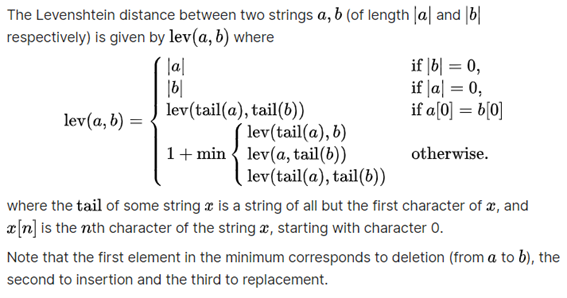
\includegraphics[width=0.48\textwidth]{figure/levenshtein.png}
            \end{center}
            \caption{Replace this part with text}
            \label{fig:wiki}
        \end{figure}

        【Replace this part with something from another paper to increase cites】

        (\url{https://en.wikipedia.org/wiki/Levenshtein_distance})

    \subsection{Difflib}
        This module provides classes and functions for comparing sequences. It can be used for example, for comparing files, and can produce difference information in various formats, including HTML and context and unified diffs. For comparing directories and files, see also, the filecmp module.
        
        【Replace this part with something from another paper to increase cites】

        (\url{https://python.readthedocs.io/en/latest/library/difflib.html})
    
    \subsection{FuzzyWuzzy}
        FuzzyWuzzy is a Python library useing Levenshtein Distance to calculate the differences between sequences. It relies on the Difflib module.

        【Replace this part with something from another paper to increase cites】

        (\url{https://chairnerd.seatgeek.com/fuzzywuzzy-fuzzy-string-matching-in-python/})
        
        (https://github.com/seatgeek/fuzzywuzzy)

\section{Proposal of Speed-up Method}
\label{sec:algorithm}
    In this section, we propose the speed-up method for the Fuzzy search process in the product label recognition system.

    \subsection{Proposal Overview}
        In the proposal, first, optical character recognition (OCR) is used to convert the picture into text. Second, we use a regular expression to filter and extract all alphanumeric strings which have possibility to be model text from the OCR recognition result. Then, we split the alphanumeric strings into two halves, and use partial word matching to pick model texts containing either half from the master database, which is pre-prepared and contains a large number of product models. Finally, we do fuzzy search in all the models picked, to find model texts most similar to any of the alphanumeric strings, which are the most possible real model. 
        
    \subsection{OCR Text Processing with Regular Expression}
    \label{sec:algorithm.ocrregex}
        In the process of extracting model info from OCR processed text from product label, we firstly use a regular expression to recognize the guidance keywords like {\em Model}, {\em Catalog}, etc. But when tested in practice, we found the recognition rate unfavorable. The result is shown in table \ref{table:regex}.
        
        The regular expression we use (letter case ignored):

        \begin{center}
        \begin{BVerbatim}
((MODEL|Model)([^\.:\n]*[\.: \n]+)|(形名|型名|型番
|品番|モデル)([^\.:\n]*[\.: \n]+)?)(\n?[ a-zA-Z0-9
\-\/\(\)]*[0-9][ a-zA-Z0-9\-\/\(\)]*)[ \n]
        \end{BVerbatim}
        \end{center}

        \begin{table}[tb]
            \caption{OCR text processing with regular expression test results}
            \label{table:regex}
            \begin{center}
                \begin{tabular}{c|>{\centering\arraybackslash}p{2cm}}
                \Hline
                Item & Count \\ 
                \Hline
                Photos Tested & 177 \\
                Correct Recognition & 51 \\
                Incorrect Recognition & 126 \\
                \hline
                Recognition Rate (\%) & 28.81 \\
                \Hline
                \end{tabular}
            \end{center}
        \end{table}

        Because of the technical limitations in OCR, the recognized text cannot be 100\% accurate. As the brightness, contrast, or other environmental condition when the pictures of product labels are taken changes, the accuracy of recognition can fluctuate significantly. The material or color of the product label can also perform great influence on the recognition results.
        
        \begin{figure}[t] 
            \begin{center}
            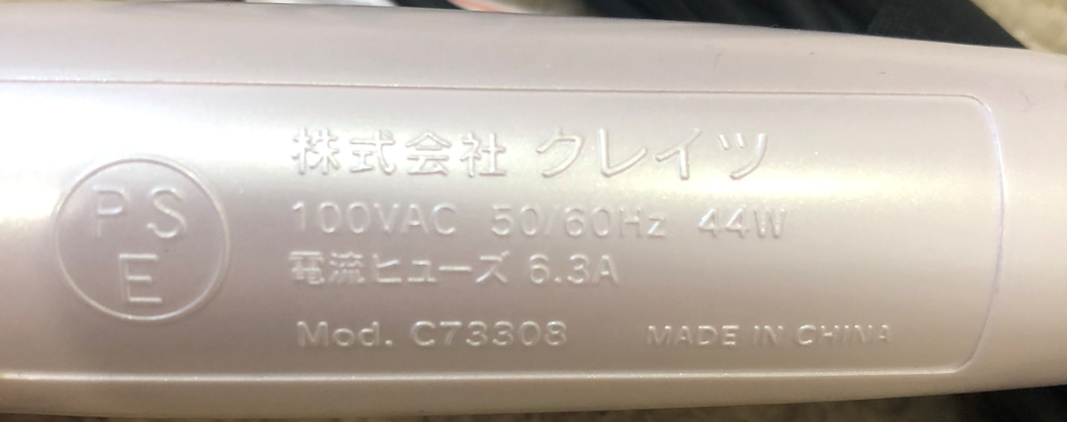
\includegraphics[width=0.48\textwidth]{figure/plastic.png}
            \end{center}
            \caption{A label with protruding texts directly engraved on the plastic case}
            \label{fig:plastic}
        \end{figure}

        In the label in figure \ref{fig:plastic}, the protruding texts are directly engraved on the plastic case. The foreground is the same color as the background, so it is difficult to recognize all the text correctly.
        
        Also, for some similar characters it is very hard for OCR to tell apart, like letter “O” and number “0”, letter “l” and number “1”. In the picture in figure \ref{fig:letter-number}, the number 0 in model, which is in the top left corner was incorrectly recognized as letter O. 
        
        \begin{figure}[t] 
            \begin{center}
            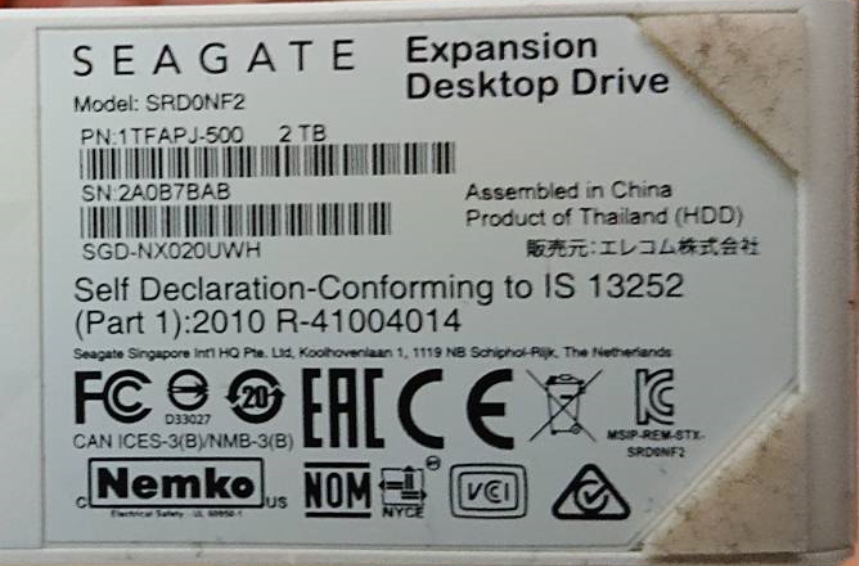
\includegraphics[width=0.48\textwidth]{figure/letter-number.png}
            \end{center}
            \caption{A label with misrecognized number 0}
            \label{fig:letter-number}
        \end{figure}

        Model text are mostly irregular alphanumeric strings rather than meaningful English words. Thus, it is also hard to use OCR error correction basing on word classification.
        
        \vspace*{\baselineskip}

        【insert something from paper to increase cites】\\
        (https://arxiv.org/ftp/arxiv/papers/1604/1604.06225.pdf)

        \vspace*{\baselineskip}
        
        Also, like in figure \ref{fig:3models}, there are some labels containing multiple guidance keywords. For example having both {\em Model Name} and {\em Model No.} in English, together with {\em 型番} in Japanese which also means model.

        \begin{figure}[t] 
            \begin{center}
            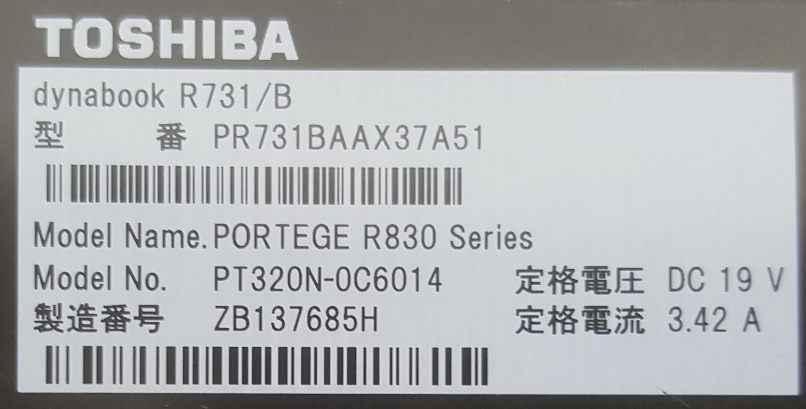
\includegraphics[width=0.48\textwidth]{figure/3models.png}
            \end{center}
            \caption{A label containing multiple guidance keywords}
            \label{fig:3models}
        \end{figure}

        Furthermore, the guidance keywords we used for regular expression recognition do not exist on some of the labels we tested. On these labels, such as in figure \ref{fig:no-guidance.png}, alphanumeric product models are just printed in different fonts or sizes, sometimes even the same appearance as other texts in the same label. Recognition could be difficult because such appearance information is lost after OCR.
        
        \begin{figure}[t] 
            \begin{center}
            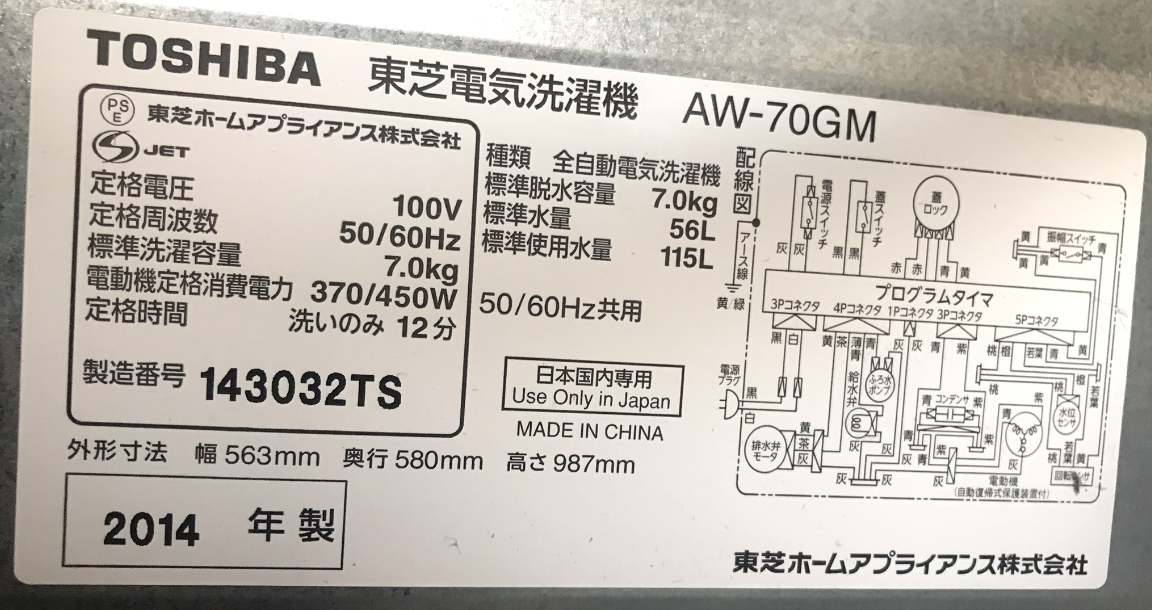
\includegraphics[width=0.48\textwidth]{figure/no-guidance.png}
            \end{center}
            \caption{A label with no guidance keywords}
            \label{fig:no-guidance.png}
        \end{figure}

        Thus, processing OCR text results with regular expression specialized in recognizing guidance keywords is not very reliable. We need some other additional solutions together to improve the accuracy.
        
    
    \subsection{Word Matching from Master Database}
        In view of the limited accuracy of OCR-based regular expression recognition, in order to improve the accuracy, we use a pre-prepared master database containing a large number of product models to perform text matching queries.
        
        In order to identify product labels that do not have guidance keywords and directly print alphanumeric strings on its surfaces, we first use regular expressions to extract all alphanumeric strings which have possibility to be Model text in the OCR recognition result. The test result is shown in table \ref{table:word-matching}.
    
        The regular expression we use:

        \begin{center}
        \begin{BVerbatim}
[ :]*(([a-zA-Z0-9\-\/\(\)]{4,} (?=[ a-zA-Z
0-9\-\/\(\)]*[0-9])[ a-zA-Z0-9\-\/\(\)]+)|
((?=[a-zA-Z0-9\-\/\(\)]*[0-9])[a-zA-Z0-9\-
\/\(\)]{4,}))[ ,.]*
        \end{BVerbatim}
        \end{center}

        \begin{table}[tb]
            \caption{Word matching from master database test results}
            \label{table:word-matching}
            \begin{center}
                \begin{tabular}{c|>{\centering\arraybackslash}p{2cm}}
                \Hline
                Item & Count \\ 
                \Hline
                Photos Tested & 177 \\
                Correct Recognition & 150 \\
                Incorrect Recognition & 27 \\
                \hline
                Recognition Rate (\%) & 84.75 \\
                \Hline
                \end{tabular}
            \end{center}
        \end{table}

        On this basis, we query the possible model texts from all the product models in the master database using full word matching, and extract the correct product model result, as candidate results to output.
    
        \vspace*{\baselineskip}
        [Figure: The matched results]
        \vspace*{\baselineskip}
    
        Using this method, as long as the master database with a large enough coverage is prepared in advance, the probability of the model being correctly identified can be greatly improved.
        
        However, this method is still limited, and it cannot solve the recognition errors that inevitably occur in the OCR process. As mentioned earlier in chapter \ref{sec:algorithm.ocrregex}, OCR error correction for irregular alphanumeric model texts has very limited effect. For the model text with recognition error, even if our regular expression can successfully recognize it as a candidate string, the whole word matching query from the master DB will still fail.
    
        \vspace*{\baselineskip}
        [Figure: A text with one incorrect letter recognition and its photo]
        \vspace*{\baselineskip}
    
    \subsection {Non-Limit Fuzzy Search}
        In order to tolerate OCR recognition errors to a certain extent, we give up whole word matching and instead use Fuzzy Search for master database search. Specifically in this proposal, we use {\em FuzzyWuzzy} to calculate the similarity between two strings.
        
        The similarity is an integer ranging from 0 to 100. When two strings are exactly the same, the similarity is 100. When a recognition error occurs, for a common 5-character model string, take the amount of character error as 1, as shown in figure \ref{fig:code_fuzzwuzzy}, the similarity is 80.
        
        \begin{figure}[tb]
            \begin{lstlisting}
>>> from fuzzywuzzy import fuzz
>>> fuzz.ratio("A1532", "A15B2")
80          \end{lstlisting}
            \caption{The similarity of a 5-character string with 1-character error}
            \label{fig:code_fuzzwuzzy}
        \end{figure}
        
        For the OCR errors of model text, in the 300 (要修正) test cases we conducted, there were 10 (要修正) times that 1 character was incorrectly recognized, and there was no case with more than 2 recognition errors. Therefore, it can be considered that in most cases, the number of incorrectly recognized characters will not exceed one.
        
        With Fuzzy Search, for each identified alphanumeric string that may be model text, we compare it with all the model texts recorded in the master database, to calculate their similarity. The several matching results (5 by default) with highest similarity among all results are taken as candidates for output, which can ensure a higher accuracy.
        
        As shown in Table \ref{table:non-limited}, in our test, among 300 (要修正) test cases with a master database covering all the correct models from the picture were performed, of which 290 (要修正) cases can output the correct model in the first candidate of the matching list, and 9 times (要修正)in the second candidate. The recognition rate has reached 99.67\%.
        
        \begin{table}[tb]
            \caption{Non-Limit Fuzzy Search test results}
            \label{table:non-limited}
            \begin{center}
                \begin{tabular}{c|>{\centering\arraybackslash}p{2cm}}
                \Hline
                item & count \\ 
                \Hline
                test cases & 300 \\
                1st correct candidates & 290 \\
                2nd correct candidates & 9 \\
                correct candidates & 299 \\
                \hline
                successful recognition rate (\%) & 99.67 \\
                \Hline
                \end{tabular}
            \end{center}
        \end{table}
    
    
    \subsection{Fuzzy Search Limited by Partial Word Matching}
        In this subsection, we describe the details of the proposal of fuzzy search limited by partial word matching.
        
        \subsubsection{Forward Matching and Backward Matching}
            Although the aforementioned Fuzzy Search method effectively improves the recognition accuracy, the search complexity is O(n). With one more possible alphanumeric string added, its similarity calculation with all the model texts in the database is required. If the number of model texts in the master database also increases, the calculation amount will increase considerably. Fuzzy Search takes about (?) times the time required for full word matching search.
            
            In our test environment, there are about 550,000 models recorded in the master database. For a single search with 15 possible alphanumeric strings, {\em 15 × 550,000 = 8,250,000} searches and similarity calculations are required. This can take up to several minutes, and it is difficult to use it in a production environment to provide services to users.
            
            Therefore, we perform a search range limitation before conducting Fuzzy Search. For each possible alphanumeric string, the query and calculation from all the model texts in the master database are not performed directly. Instead, the search range is limited according to other restrictions, thereby reducing the total amount of calculation and time-consuming.
            
            As in one alphanumeric string, in most cases, there will be no more than 1 OCR error, we divide one alphanumeric string into two halves. For each half, forward matching or backward matching is performed.
            
            In this way, if the misrecognized character is in the second half, the first half is a correct recognition. Forward matching can ensure that the completely matched correct model from the master database is included in the matching result. Conversely, if the misrecognized character is in the first half, backward matching can help us to match the correct model.
            
            Let the original label text be “MX1234567” and the OCR result be “MX12345b7”, with one error. As shown in table \ref{table:half_matching}, it is divided into “MX123” and “45b7”. The matching result will contain the correct “MX1234567” model and together with some other models sharing the same half.

            \begin{table}[tb]
                \caption{Half divided string and its matching results}
                \label{table:half_matching}
                \begin{center}
                    \begin{tabular}{c|c|c}
                    \Hline
                    origional label text & \multicolumn{2}{c}{MX1234567} \\ 
                    \hline
                    OCR result & \multicolumn{2}{c}{MX12345{\em b}7} \\ 
                    \hline
                    half divided strings & MX123\_\_\_\_ & \_\_\_\_45{\em b}7 \\
                    \hline
                    matching results & \begin{tabular}{c}MX123\underline{4567}\\MX123\underline{5678}\\...\end{tabular} & (no result)) \\
                    \Hline
                    \end{tabular}
                \end{center}
            \end{table}
            
            List all the matching results obtained by this matching method, within this range, perform the Fuzzy Search described above. After this half matching, the search range of Fuzzy Search can be greatly limited, and the amount of query and calculation can be reduced.
        
        \subsubsection{Partial Word Matching}
            Considering that the recognition error of OCR may not only cause text replacement, but also cause text missing at the beginning or end. As an improvement, forward matching and backward matching are replaced into partial word matching, that is, as long as the model text in the master database contains one half of the recognized alphanumeric strings as a substring, it will be added to the search range for Fuzzy Search. This processing method will slightly increase the search range, but the order of magnitude of the amount of model texts included in the search range generally does not change.
    
\section{Evaluation}
\label{sec:evaluation}
    In this section, we evaluate the proposal. 
    
    We conducted 300 searches in a master database with 550,000 records. The time consumed is shown in the table \ref{table:methods_compare}.
    
    \begin{table*}[t]
        \caption{Performance result using different searching methods [DATA NEEDS CORRECTION]}
        \label{table:methods_compare}
        \begin{center}
            \begin{tabular}{c|cccc}
            \Hline
            search method &
                \begin{tabular}{c}regular expression\\Recognition with\\Guidance Keywords\end{tabular} &
                \begin{tabular}{c}Full Word Matching\\with master DB\end{tabular} &
                \begin{tabular}{c}Non-Limit\\Fuzzy Search\end{tabular} &
                \begin{tabular}{c}Fuzzy Search\\Limited by Partial\\Word Matching\end{tabular} \\ 
            \hline
            1st candidate in matching list was correct &
                 & & 290 & \\ 
            \hline
            2nd candidate in matching list was correct &
                N/A & N/A & 9 & \\ 
            \hline
            Recognition Rate &
                 & & 99.67\% & \\ 
            \hline
            Average Search Time &
                 & & 120s & 0.13s \\ 
            \hline
            Maximum Search Time &
                 & & 180s & 13s \\ 
            \hline
            Average Search Range (DB Record Amount) &
                N/A & 550,000 & 550,000 & 3,000 \\
            \Hline
            \end{tabular}
        \end{center}
    \end{table*}
    
    Among the Fuzzy Search limited by partial word matching results, the several experiments in which the time-consuming is significantly higher than the average time-consuming are as in the table \ref{table:slowest_rec}.

    \begin{table*}[t]
        \caption{Performance result using different searching methods [DATA NEEDS CORRECTION]}
        \label{table:slowest_rec}
        \begin{center}
            \begin{tabular}{c|c|c|c|c|c|c}
            \Hline
            No. &
                Real Product Model &
                \begin{tabular}{c}Query Alphanumeric\\String (OCR result)\end{tabular} &
                \begin{tabular}{c}Limiting Time\\(Partial Word Matching\\Costed Time)\end{tabular} &
                \begin{tabular}{c}Fuzzy Search\\Costed Time\end{tabular} &
                \begin{tabular}{c}Fuzzy Search Range\\(DB Record Amount)\end{tabular} &
                \begin{tabular}{c}Total Costed Time\end{tabular} \\ 
            \Hline
            1 & & & & & & \\ 
            \hline
            2 & & & & & & \\ 
            \Hline
            \end{tabular}
        \end{center}
    \end{table*}
    
    \section{Related Works}
    \label{sec:related}
        In this section, we introduce related works to the proposal.
        
        % In \cite{related1}, Kashihara et al. proposed a method of blanking an important point of data or control flow in a C code using {\em Program Dependence Graph (PDG)}, to make instructive fill-in-blank problems without considering semantic aspects. PDG can represent the relationship of data dependency and control flows between commands using a graph.
        
        % In \cite{related2}, Shinkai et al. provided a C programming education assistant system on {\em Moodle} using fill-in-blank problems like in this paper. It extracts important elements in a code for questions using PDG.
        
        % In \cite{related3}, Terada et al. proposed a methodology to automatically generate fill-in-blank problems for C codes. To automatically generate problems, two key constituents, the selection of exemplary code and the selection of places to be blanked, are presented. For the first one, they use k-means clustering with silhouette analysis is used to select exemplary code from the Aizu Online Judge system (AOJ) which has over 3 million of source codes. For the later one, a model based on a bidirectional {\em Long Short-Term Memory Network (Bi-LSTM)} with a sequential {\em Conditional Random Field (CRF)} is used.
        
    \section{Conclusion}
    \label{sec:conclusion}
        It can be seen that using Fuzzy Search Limited by Partial Word Matching can effectively reduce the time into the acceptable range while increasing the accuracy rate to be close to that of Non-Limit Fuzzy Search. With this method, we can take a balance between searching speed and mistake prevention for OCR text, and successfully limit the search range into several thousand (about 0.3\% of all data amount). In most cases the search result would come out in only less than 1 second which is acceptable for users to wait. This method turns out to be possible to put into practice when deploying into web services.
        
        It can be seen from the experimental data that for rare cases, after the limitation of character recognition, the search range is still large.
        
        We consider that, for each record in the master database, it not only contains the model text information of the product, but also its brand or manufacturer information. Before doing Fuzzy Search, we can also use other recognition methods to match and analyze the text contained in the OCR results to determine the brand of the product, and use brand information matching to further limit the search range of Fuzzy Search for model texts, which may further improve searching performance.
        

%\bibliographystyle{sieicej}
%\bibliography{myrefs}
\begin{thebibliography}{99}% 文献数が10未満の時 {9}
    \bibitem{popularity}
    \url{https://www.spectrum.ieee.org/at-work/tech-careers/top-programming-language-2020}

    \bibitem{Funabiki13} 
    N. Funabiki, Y. Matsushima, T. Nakanishi, and N. Amano, "A Java programming learning assistant system using test-driven development method," \emph{IAENG Int. J. Comput. Sci.}, vol. 40, no.1, pp. 38-46, Feb. 2013.
    
    \bibitem{Zaw15}
    K. K. Zaw, N. Funabiki, and W.-C. Kao, "A proposal of value trace problem for algorithm code reading in Java programming learning assistant system," \emph{Inf. Eng. Express}, vol. 1, no. 3, pp. 9-18, Sep. 2015.
    
    \bibitem{Funabiki17} 
    N. Funabiki, Tana, K. K. Zaw, N. Ishihara, and W.-C. Kao, "A graph-based blank element selection algorithm for fill-in-blank problems in Java programming learning assistant system, \emph{IAENG Int. J. Comput. Sci.}, vol. 44, no. 2, pp. 247-260, May 2017.
    
    \bibitem{cup}
    CUP, \url{http://czt.sourceforge.net/dev/java-cup/manual.html}
    
    \bibitem{scope}
    Scope, https://www.codesdope.com/blog/article/scope-of-variables-in-c/
    
    \bibitem{example}
    \url{http://www.codebind.com/c-examples/}
    
    \bibitem{triangle}
    \url{https://brilliant.org/wiki/pascals-triangle/}
    
    \bibitem{related1}
    A. Kashihara, A. Terai, and J. Toyota, "Making fill-in-blank program problems for learning algorithm, " \emph{in Proc. Int. Conf. Comput. Edu.}, pp. 776-783, 1999.
    
    \bibitem{related2}
    J. Shinkai, Y. Hayase, and I. Miyaji, "A study of generation and utilization of fill-in-the-blank questions for programming education on Moodle, " \emph{IEICE Technical Report}, vol. 110, no. 263, pp. 7-10, 2010.
    
    \bibitem{related3}
    K. Terada, Y. Watanobe, "Automatic generation of fill-in-the-blank programming problems, " \emph{in Proc. IEEE Int. Symp. Embed. Mult./Many-core Sys.-on-Chip (MCSoC)}, pp. 187-193, 2019.
\end{thebibliography}

\end{document}
